\subsection{Analysis}

For the concept wise performance of the \textit{CoAtt} models, it is observed that the performance is more uniform throughout the concepts as compared to more varied distribution of the subsequence model. For concepts like WHAT, WHO, WHERE, HOW, THERE where the subsequence model performed poorly, the \textit{CoAtt} model is able to acheive high scores. The \textit{CoAtt} model performs poorly on a few selected concepts like AT, IF, IN, BECAUSE, GIVE. By looking at the samples, it is found that these concepts are heavily biased by negative samples and contain only a handful of positive cognate pair examples. In fact the subsequence model could not perform at all on these concepts as the highly biased data is coupled with almost no overlap of subsequences.

\begin{table}[h]
\centering
	\begin{minipage}{.5\linewidth}
      \centering

\begin{tabular}{ccc}
\textbf{Concept} & \textbf{CoAtt} & \textbf{Subseq} \\ \hline
WHAT             & \textit{0.91}  & \textit{0.04}   \\
WHO              & \textit{0.85}  & \textit{0.05}   \\
WHERE            & \textit{0.90}  & \textit{0.16}   \\
HOW              & \textit{0.90}  & \textit{0.17}   \\
THERE            & \textit{0.95}  & \textit{0.19}  
\end{tabular}


	\end{minipage}%
    \begin{minipage}{.5\linewidth}
    \centering

\begin{tabular}{ccc}
\textbf{Concept} & \textbf{CoAtt} & \textbf{Subseq} \\ \hline
BECAUSE          & \textit{0.28}  & \textit{0}      \\
IN               & \textit{0.35}  & \textit{0}      \\
IF               & \textit{0.31}  & \textit{0}      \\
AT               & \textit{0.25}  & \textit{0}      \\
GIVE             & \textit{0.45}  & \textit{0.35}  
\end{tabular}

	\end{minipage} 
\caption{\textit{CoAtt} vs \textit{Subseq} model on various concepts (F-Score)}
\end{table}

To compare the IPA model with the ASJP models on the IELex dataset, it is found that the IPA model performs poorly on concepts like GUTS, SWIM, WIPE, WHITE, SING where the ASJP model gives good results. On the other hand, the IPA model performs better on concepts like FIRE, SLEEP, PULL, SAY and SMOOTH. By looking at specific examples, we find that for concepts like FIRE and PULL, the ASJP model gives many false positives which can be a fault due to the coarser representation of the ASJP character.

\begin{table}[h]
\centering
	\begin{minipage}{.5\linewidth}
      \centering

\begin{tabular}{ccc}
\textbf{Concept} & \textbf{IPA}  & \textbf{ASJP} \\ \hline
GUTS             & \textit{0.28} & \textit{0.58} \\
SWIM             & \textit{0.47} & 0.93          \\
WHITE            & \textit{0.54} & \textit{0.75} \\
WIPE             & \textit{0.55} & \textit{0.72} \\
SING             & \textit{0.56} & \textit{0.88}
\end{tabular}

	\end{minipage}%
    \begin{minipage}{.5\linewidth}
    \centering

\begin{tabular}{ccc}
\textbf{Concept} & \textbf{IPA}  & \textbf{ASJP} \\ \hline
FIRE             & \textit{0.62} & \textit{0.33} \\
SLEEP            & \textit{0.73} & 0.39          \\
PULL             & \textit{0.83} & \textit{0.50} \\
SMOOTH           & \textit{0.83} & \textit{0.50} \\
SAY              & \textit{0.90} & \textit{0.51}
\end{tabular}

	\end{minipage} 
\caption{\textit{CoAtt} model using IPA vs ASJP transcription on various concepts (F-Score)}
\end{table}

\clearpage
Figure 5-5 shows few test sample pairs from the concept SWIM. It is observed that for all of these samples, the IPA model falsely predicts negatives whereas the ASJP model is correctly able to predict them all as cognates. Here perhaps the very find representation in IPA throws the model's judgment off and its not able to pick up the correspondence correctly. It is also interesting to note that for all of these samples, adding the \textit{concept feature} of SWIM to the \textit{CoAtt + Concept Features} model makes it predict all of them as cognates. Thus, perhaps adding the concept features signals the model to relax the degree of overlapping of phonemes and become less strict in predicting cognates.

\begin{figure}[t]
\centering
  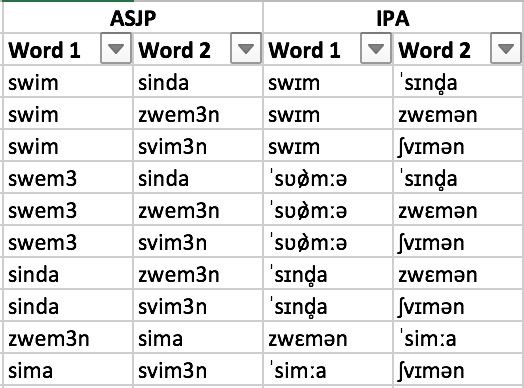
\includegraphics[width=.5\linewidth]{swim}
  \caption{Sample test word pairs from the concept SWIM}
  \label{disssim}
\end{figure}

\subsection{Hindi-Marathi Extractions}

Finally we applied the \textit{CoAtt} model to the domain of Hindi-Marathi. The model was trained on the IELex dataset with IPA transcription with a character vocabulary of around 150 phonetic characters. The model was trained in a cross-language evaluation style. It should be noted that the IELex database contains instances from Marathi, but it does not directly contain instances from Hindi. However, it does contain words from Urdu and Bhojpuri (Bihari) which are also languages closely related to Hindi and share many words of the vocabulary with Hindi.

We used the TDIL sentence-aligned corpus. The corpus contains sentences from Hindi-Marathi that are POS tagged and transcribed in Devanagari. We specifically extracted word pairs from each sentence with the NOUN and VERB tags. Since the sentences are not word aligned, we extracted candidate word pairs for testing by choosing the first word with the same tag in either sentence as the candidate pair. The words were converted from Devanagari to IPA using a rule-based system and finally fed into the model. We extracted 16K pairs from Nouns and 9K pairs from Verbs.

Some randomly sampled extractions from the test samples are shown in the figures. On first observation it seems that the model is doing a fair job of aligning similar word pairs that are possibly cognates. We plan to do further manual evaluation of these extraction. The model is able to find word pairs with a common stem without the need of lemmetization. In the case of verbs, it can be observed that the model is able to see through the inflections on the verbs to predict the pairs with similar stems as cognates. Figure \ref{disssim} is most illustrative of the ability of the model. It presents few exceptional cases where the word pairs predicted as cognates are not straightforwardly similar.

\begin{figure}[ht]
\centering
\begin{subfigure}{.5\textwidth}
  \centering
  \includegraphics[width=.65\linewidth]{nn_1}
  \caption{Positive Label}
\end{subfigure}%
\begin{subfigure}{.5\textwidth}
  \centering
  \includegraphics[width=.65\linewidth]{nn_0}
  \caption{Negative Label}
\end{subfigure}
\caption{Hindi-Marathi Noun Pairs}
\end{figure}

\begin{figure}[ht]
\centering
\begin{subfigure}{.5\textwidth}
  \centering
  \includegraphics[width=.65\linewidth]{vbs_1}
  \caption{Positive Label}
\end{subfigure}%
\begin{subfigure}{.5\textwidth}
  \centering
  \includegraphics[width=.65\linewidth]{vbs_0}
  \caption{Negative Label}
\end{subfigure}
\caption{Hindi-Marathi Verb Pairs}
\end{figure}

\begin{figure}[ht]
\centering
  \includegraphics[width=.65\linewidth]{dissim}
  \caption{Positive Label Noun Pairs Exceptional Cases}
  \label{disssim}
\end{figure}
